% 2000 年全国新课程卷文科第 18 题甲：直三棱柱 ABC-A_1B_1C_1
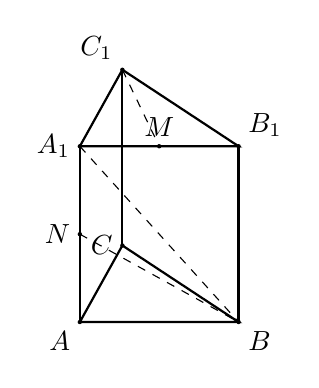
\begin{tikzpicture}[>=stealth, scale=0.72]
  \coordinate (A) at (0,0);
  \coordinate (B) at (2.8,0);
  \coordinate (C) at (0.75,1.35);
  \coordinate (A1) at (0,3.1);
  \coordinate (B1) at (2.8,3.1);
  \coordinate (C1) at (0.75,4.45);
  \coordinate (M) at (1.4,3.1);
  \coordinate (N) at (0,1.55);

  \draw[thick] (A)--(B)--(C)--cycle;
  \draw[thick] (A1)--(B1)--(C1)--cycle;
  \draw[thick] (A)--(A1) (B)--(B1) (C)--(C1);
  \draw[dashed] (A1)--(B) (C1)--(M) (N)--(B);

  \fill (A) circle (1.1pt) node[below left] {$A$};
  \fill (B) circle (1.1pt) node[below right] {$B$};
  \fill (C) circle (1.1pt) node[left] {$C$};
  \fill (A1) circle (1.1pt) node[left] {$A_1$};
  \fill (B1) circle (1.1pt) node[above right] {$B_1$};
  \fill (C1) circle (1.1pt) node[above left] {$C_1$};
  \fill (M) circle (1.1pt) node[above] {$M$};
  \fill (N) circle (1.1pt) node[left] {$N$};
\end{tikzpicture}
